\chapter{Padrões Comportamentais}

\section{Chain of Responsibility}

Chain of Responsability propõe criar uma estrutura para 
tratar solicitações feitas por um objeto cliente. As classes 
que tratam as solicitações são chamadas de \textit{handlers}. 
Uma solicitação é passada adiante por uma cadeia de 
\textit{handlers} até que seja tratada ou 
até que a cadeia chegue ao fim e a solicitação 
não possa ser atendida, retornando uma indicação 
de que a solicitação não pôde ser atendida.

Essa abordagem permite desacoplar os clientes das classes 
que tratam as solicitações e permite que os \textit{handlers} 
sejam definidos dinamicamente. Por outro lado, pode não ser 
possível prever se uma solicitação de um cliente será atendida, 
caso o \textit{handler} adequado não esteja na cadeia. A 
estrutura do padrão pode ser vista na figura \ref{chain_struct}.

\begin{figure}[htb]
	\caption{\label{chain_struct}Estrutura do Chain of Responsibility}
	\begin{center}
	    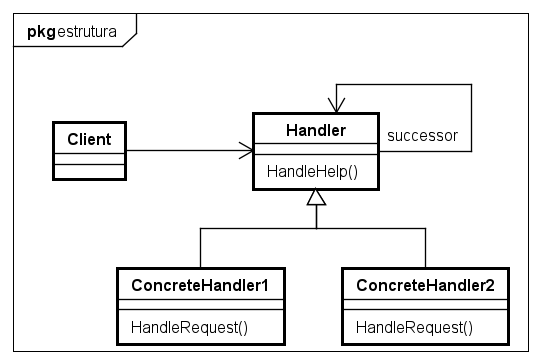
\includegraphics[scale=0.5]{5_padroes-contexto-funcional/5.3_comportamentais/5.3.01_chain-of-responsibility/chainofresponsibility_struct.png}
	\end{center}
\end{figure}

\subsection*{Exemplo Orientado a Objetos}

O exemplo do Chain of Responsibility traz um recurso 
de \textit{help} utilizado nos componentes de uma 
interface gráfica. O recurso é sensível ao contexto, 
bastando que o usuário solicite a ajuda no local 
desejado. O objeto que fornece a ajuda não é 
conhecido pelos objetos dos \textit{widgets} da 
interface, ele pertence a uma cadeia que é 
percorrida sempre que o usuário solicita 
a ajuda. A figura \ref{chain_exemplo} e o código 
\ref{oochresponsibility} demonstram esse exemplo.

\begin{figure}[htb]
	\caption{\label{chain_exemplo}Exemplo de Chain of Responsibility}
	\begin{center}
	    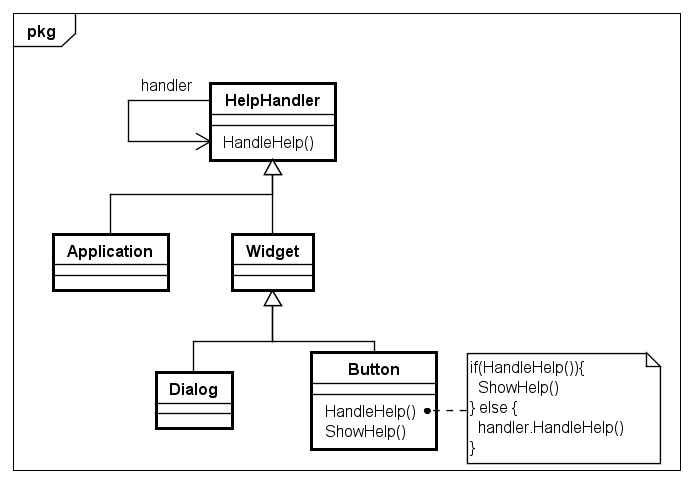
\includegraphics[scale=0.5]{5_padroes-contexto-funcional/5.3_comportamentais/5.3.01_chain-of-responsibility/chainofresponsibility_exemplo.png}
	\end{center}
\end{figure}

\begin{lstlisting}[caption={Chain of Responsibility Orientação a Objetos},label=oochresponsibility]

class HelpHandler(handler: HelpHandler = null, topic : Topic.Value = Topic.NO_HELP_TOPIC) {

  private var _handler : HelpHandler = handler
  private var _topic : Topic.Value = topic

  def HasHelp(): Boolean = {
    _topic != Topic.NO_HELP_TOPIC
  }

  def SetHandler(handler : HelpHandler, topic : Topic.Value) : Unit = {
    this._handler = handler
    this._topic = topic
  }

  def HandleHelp() : Unit = {
    if(_handler != null){
      _handler.HandleHelp()
    }
  }
}

class Widget(parent : Widget, topic : Topic.Value = Topic.NO_HELP_TOPIC)
  extends HelpHandler(parent, topic)
  
class Button(parent : Widget, topic: Topic.Value = Topic.NO_HELP_TOPIC)
  extends Widget(parent, topic) {

  override def HandleHelp(): Unit = {
    if(HasHelp()){
      //Oferece ajuda sobre o botão
    } else {
      parent.HandleHelp()
    }
  }
}

class Dialog(handler : HelpHandler, topic : Topic.Value = Topic.NO_HELP_TOPIC)
  extends Widget(null) {

  SetHandler(handler, topic)

  override def HandleHelp(): Unit = {
    if(HasHelp()) {
      // Oferece ajuda sobre dialog
    } else {
      handler.HandleHelp()
    }
  }
}

class Application(topic: Topic.Value)
  extends HelpHandler(null, topic) {

  override def HandleHelp(): Unit = {
    //Apresenta uma lista de tópicos de ajuda
  }
}

\end{lstlisting}

\subsection*{Contexto Funcional}

\begin{comment}
Dependendo da abordagem do problema, alguns tipos de Monads 
podem ser usados para resolvê-lo. Basta encapsular a 
solicitação em um Monad e fazê-la passar pelos Handlers, que 
agora seriam funções, até que a solicitação seja tratada. Em 
um exemplo em que é desejado que a cadeia de solicitação seja 
interrompida assim que um problema for encontrado, a opção 
mais indicada é o Monad Option. Um Option pode retornar algum 
valor (Some x) ou nenhum valor (None). Se alguma das operações 
retornar None, a cadeia é interrompida e os handlers 
seguintes não são executados.
\end{comment}

\begin{lstlisting}[caption={Chain of Responsibility Funcional},label=fpchresponsibility]
    

    
\end{lstlisting}